% shmap-rs -- two-page applications note.
%
% THE PROSE OF THIS FILE CONTAINS NO NUMERALS. Every measured quantity is a
% \shm... macro defined in generated/macros.tex by benchmarks/scripts/manuscript.py
% from the promoted result sets, and every table and figure is \input from
% generated/, written by paper.py and crossarch.py from the same sets. A
% benchmark run therefore rewrites this paper; nobody re-types a number into it.
%
%   python3 benchmarks/scripts/manuscript.py          refresh the macros
%   python3 benchmarks/scripts/manuscript.py --lint   catch a hand-typed number
%   python3 benchmarks/scripts/build_paper.py         typeset to manuscript.pdf
%
% A line genuinely needing a digit that is not a measurement ends with
% `% lint-ok: <reason>`. The reason is required.
%
% The two-page budget is enforced by build_paper.py, not merely intended. If a
% re-measurement pushes it over, cut prose -- the floats are generated and are
% the evidence, so they are not the place to save space.
%
% TO FILL IN BEFORE SUBMISSION: co-authors and affiliations below, and the
% final venue of the map-shmap reference, which is a draft at the time of
% writing (see QUESTIONS.md, "Open with Pesho").

\documentclass[10pt,a4paper,twocolumn]{article}

% No font package. mathptmx was tried and silently made things worse: this
% engine's bundle has no bold Times at these sizes, so every \textbf fell back
% to regular and the PDF carried not one bold glyph. Latin Modern is complete.
\usepackage[margin=1.7cm]{geometry}
\setlength{\columnsep}{0.7cm}
\usepackage{booktabs}
\usepackage{pgfplots}
\pgfplotsset{compat=1.18}
\usepgfplotslibrary{fillbetween}
\usepackage{hyperref}
\hypersetup{colorlinks=true,linkcolor=blue!45!black,urlcolor=blue!45!black,
            citecolor=blue!45!black}

% Tighter section headings than article's default, which are sized for a
% document with room to breathe. No package: \@startsection is the documented
% way and adds no dependency for build_paper.py's engine to fetch.
\makeatletter
\renewcommand\section{\@startsection{section}{1}{0pt}%
  {2.0ex \@plus .3ex \@minus .2ex}{0.6ex \@plus.2ex}{\normalsize\bfseries}}
\makeatother

% Float placement, loosened. article's defaults reserve a fifth of every page
% for text, which in a two-page note is enough to push a generated figure onto
% a third page of its own -- the exact failure build_paper.py refuses. The
% floats here ARE the evidence, so they get the room.
\renewcommand{\topfraction}{0.92}
\renewcommand{\bottomfraction}{0.70}
\renewcommand{\textfraction}{0.06}
\renewcommand{\floatpagefraction}{0.75}
\setcounter{topnumber}{2}
\setcounter{totalnumber}{3}

% Resolve \input against the generated trees, so this file typesets both from
% the repository root and from paper/ -- and so build_paper.py, which works in
% a scratch directory of copies, does not need a different draft.
\makeatletter
\def\input@path{{generated/}{generated/cross-arch/}%
                {paper/generated/}{paper/generated/cross-arch/}{./}}
\makeatother

% GENERATED by benchmarks/scripts/manuscript.py -- do not edit.
% Every number the manuscript's prose quotes, as a LaTeX macro.
% set:        x86_64/current on a2 @ 18d0f83627b5 (2026-09-12)
% set:        aarch64/current on galaxy @ 18d0f83627b5 (2026-09-12)
% reference:  x86_64 (macros named ...X; ...A is aarch64)
% inputs:     sha256:d44635e56d1be819
% provenance: paper/generated/MACROS.md
%
\newcommand{\shmHostX}{a2}
\newcommand{\shmHostA}{galaxy}
\newcommand{\shmArchX}{x86\_64}
\newcommand{\shmArchA}{aarch64}
\newcommand{\shmCoresX}{64}  % cores
\newcommand{\shmCoresA}{128}  % cores
\newcommand{\shmTopologyX}{4 sockets $\times$ 16 cores, 4 NUMA nodes}
\newcommand{\shmTopologyA}{1 socket $\times$ 128 cores, 1 NUMA node}
\newcommand{\shmCommit}{18d0f83627b5}
\newcommand{\shmMeasuredX}{2026-09-12}
\newcommand{\shmMeasuredA}{2026-09-12}
\newcommand{\shmRustc}{1.97.1}
\newcommand{\shmSuiteVersion}{1.2}
\newcommand{\shmVersion}{1.5.0}
\newcommand{\shmLicense}{MPL-2.0}
\newcommand{\shmAuthors}{Dobromir Panchev \and Pesho Ivanov}
\newcommand{\shmOrcids}{Panchev 0009-0000-2636-2593; Ivanov 0000-0002-8119-3849}
\newcommand{\shmUpstream}{https://github.com/pesho-ivanov/shmap}
\newcommand{\shmContributors}{Dobromir Petrov}
\newcommand{\shmNumOptimizations}{9}
\newcommand{\shmNumExactOptimizations}{9}
\newcommand{\shmCppCommit}{63f1103}
\newcommand{\shmNumParallelOptimizations}{3}
\newcommand{\shmAblRungs}{7}
\newcommand{\shmAblNotRungs}{2}
\newcommand{\shmAblRepeats}{5}
\newcommand{\shmAblHost}{galaxy}
\newcommand{\shmAblCores}{128}  % cores
\newcommand{\shmAblThreadsMax}{8}
\newcommand{\shmAblSpeedupOne}{1.21}  % x
\newcommand{\shmAblSpeedupMax}{2.06}  % x
\newcommand{\shmAblRssRatioOne}{4.19}  % x
\newcommand{\shmAblRssRatioMax}{36.00}  % x
\newcommand{\shmAblTopStep}{parallel FASTA}
\newcommand{\shmAblTopStepPct}{24.6}  % %
\newcommand{\shmAblTopStepRow}{6}
\newcommand{\shmAblTotalX}{2.64}  % x
\newcommand{\shmAblPortX}{2.15}  % x
\newcommand{\shmAblLadderX}{1.23}  % x
\newcommand{\shmAblRssTotalX}{7.49}  % x
\newcommand{\shmAblRssPortX}{1.70}  % x
\newcommand{\shmAblRssLadderX}{4.42}  % x
\newcommand{\shmAblBuildTuningX}{---}  % x
\newcommand{\shmParamK}{25}
\newcommand{\shmParamR}{0.01}
\newcommand{\shmParamTheta}{0.4}
\newcommand{\shmParamDelta}{0.075}
\newcommand{\shmParamPhi}{0.3}
\newcommand{\shmNumBenchmarks}{9}
\newcommand{\shmNumMetrics}{3}
\newcommand{\shmNumCells}{19}
\newcommand{\shmSpeedupXMin}{2.07}  % x
\newcommand{\shmSpeedupXMax}{2.95}  % x
\newcommand{\shmSpeedupXMedian}{2.58}  % x
\newcommand{\shmSpeedupAMin}{1.75}  % x
\newcommand{\shmSpeedupAMax}{2.55}  % x
\newcommand{\shmSpeedupAMedian}{2.21}  % x
\newcommand{\shmRssRsMin}{2.57}  % GB
\newcommand{\shmRssRsMax}{2.67}  % GB
\newcommand{\shmRssCpp}{18.85}  % GB
\newcommand{\shmRssCppSpreadMB}{6}  % MB
\newcommand{\shmMinHalflen}{5}
\newcommand{\shmRssRatioMin}{7.1}  % x
\newcommand{\shmRssRatioMax}{7.3}  % x
\newcommand{\shmRssRsFloor}{1.85}  % GB
\newcommand{\shmRssRsFloorThreads}{2}
\newcommand{\shmRssRsCap}{9.12}  % GB
\newcommand{\shmRssRsCapBench}{B04}
\newcommand{\shmRssRatioCap}{2.1}  % x
\newcommand{\shmKneeThreads}{16}
\newcommand{\shmCapThreads}{64}
\newcommand{\shmScaleXKnee}{5.9}  % x
\newcommand{\shmScaleAKnee}{10.0}  % x
\newcommand{\shmScaleXCap}{6.3}  % x
\newcommand{\shmScaleACap}{12.9}  % x
\newcommand{\shmScaleXPeak}{17.9}  % x
\newcommand{\shmScaleXPeakThreads}{32}
\newcommand{\shmScaleXPeakBench}{B04}
\newcommand{\shmScaleAPeak}{28.8}  % x
\newcommand{\shmScaleAPeakThreads}{64}
\newcommand{\shmScaleAPeakBench}{B04}
\newcommand{\shmAgreeCells}{15}
\newcommand{\shmAgreeTotal}{15}
\newcommand{\shmDetChecks}{15}
\newcommand{\shmDetTotal}{15}
\newcommand{\shmAccMin}{98.76}  % %
\newcommand{\shmAccMax}{99.21}  % %
\newcommand{\shmWrongQMax}{6}  % reads
\newcommand{\shmTopStage}{map: match\_rest}
\newcommand{\shmTopStageShare}{20.8}  % %
\newcommand{\shmShiftStage}{map: match\_seeds}
\newcommand{\shmShiftPP}{9.1}  % pp
\newcommand{\shmMapRatioMin}{0.97}  % x
\newcommand{\shmMapRatioMax}{1.31}  % x


\title{\vspace{-1.0cm}\textbf{shmap-rs: exact, parallel and memory-lean
       sketch-based long-read mapping}}
% The byline comes from .zenodo.json, so the paper and the DOI cannot name
% different people. Add or reorder authors there, not here.
% TODO before submission: affiliations.
\author{\shmAuthors}
\date{}

\begin{document}
\maketitle
\vspace{-0.7cm}

\begin{abstract}
\noindent
\textbf{Summary:} \emph{map-shmap} maps long reads by comparing FracMinHash
sketches of read and reference under a seed heuristic that prunes candidate
regions before refining them. Its reference implementation is single-threaded
and sizes its bucket accumulator against the \emph{reference}, putting
whole-genome mapping outside ordinary memory budgets. We present
\textbf{shmap-rs}, a Rust implementation that leaves the algorithm untouched
--- output is byte-identical --- and rebuilds the data structures and the
parallel decomposition around it. Against the tuned C++ reference it is
\shmSpeedupXMin--\shmSpeedupXMax$\times$ faster single-threaded, uses
\shmRssRatioMin--\shmRssRatioMax$\times$ less peak memory, and adds thread
parallelism the reference lacks, reaching \shmScaleXPeak$\times$ on
\shmCoresX{} cores. Every claim is measured on two architectures, whose runs
agree on every algorithmic counter.\\[0.2em]
\textbf{Availability:} \url{https://github.com/d0bromir/shmap-rs}, \shmLicense,
version~\shmVersion. The benchmark suite, the result sets and the generators of
every table here are in the repository.\\[0.2em]
\textbf{Contact:} ORCID \shmOrcids.
\end{abstract}

\section{Introduction}

Sketch-based mappers compare a read to a genome in the space of a few thousand
hashes rather than a few billion bases~\cite{mash}.
\emph{map-shmap}~\cite{shmap} sketches read and reference by FracMinHash,
accumulates seed matches into overlapping buckets, prunes them with an
admissible seed heuristic, and refines the survivors with a sliding window. Its
cost is dominated by dependent memory references rather than arithmetic, which
is why it was worth re-engineering rather than re-designing. No change may
alter a single output record, so every number below compares two
implementations of one algorithm.

\section{Implementation}

\textbf{A bucket accumulator sized by the read, not the reference.} The
reference allocates a dense array indexed by reference bucket, so its footprint
is a property of the genome and is paid on every run. A read can only match
buckets within its own span, so shmap-rs sizes the array by the read's
half-length, falling back to a sparse map otherwise. This is almost the whole
memory result, and it removed a contention bottleneck that had made
multithreading nearly useless.

\textbf{Memoised refinement.} The second-best-mapping search repeats scoring
the best-mapping search has already done; shmap-rs replays those scores instead,
removing roughly two calls in five into refinement. It is applied only to the
metrics where replay is provably sound.

\textbf{Parallelism the reference does not have.} Reference sketching is
chunked, index storage sharded by hash, FASTA parsing a two-pass
count-then-fill. All three are parallel and none is order-dependent: the index
does not depend on how many threads built it, which is what lets output stay
byte-identical.

\textbf{Hot-loop work.} Repetitive seeds accumulate in place at constant
integer cost rather than through a scratch hash map; the rolling nucleotide
hash~\cite{nthash} keeps its rotations precomputed and its iteration free of
bounds checks; and final bucket ordering uses an unstable sort over a packed
key reproducing exactly what a stable sort would give --- the optimisation the
original paper specifies, made deterministic, which the reference's
\texttt{std::sort} does not guarantee.

Exactness is enforced, not asserted: the suite checks output is identical
across every thread count (\shmDetChecks{} of \shmDetTotal{} checks) and
against the reference, and blocks a merge on any drop in mapped or
confidently-mapped reads.

\section{Results}

{\small% GENERATED by benchmarks/scripts/crossarch.py -- do not edit.
% artifact:   table_crossarch_speedup (table)
% set:        x86_64/current on a2 @ 18d0f83627b5 (2026-09-12)
% set:        aarch64/current on galaxy @ 18d0f83627b5 (2026-09-12)
% reference:  x86_64 (every delta is against this)
% inputs:     sha256:32da7e14ac55e610
% provenance: paper/generated/cross-arch/PROVENANCE.md#table_crossarch_speedup
%
\begin{table}[tb]
\centering
\begin{tabular}{llrrr}
\toprule
Benchmark & Metric & \texttt{x86\_64} & \texttt{aarch64} & $\Delta$ \\
\midrule
B01 & Containment & 2.74$\times$ & 2.32$\times$ & -0.42 \\
B01 & Jaccard & 2.57$\times$ & 2.19$\times$ & -0.37 \\
B01 & bucket\_SH & 2.84$\times$ & 2.38$\times$ & -0.46 \\
\midrule
B02 & Containment & 2.58$\times$ & 2.40$\times$ & -0.18 \\
B02 & Jaccard & 2.31$\times$ & 2.21$\times$ & -0.10 \\
B02 & bucket\_SH & 2.65$\times$ & 2.52$\times$ & -0.13 \\
\midrule
B03 & Containment & 2.49$\times$ & 1.97$\times$ & -0.51 \\
B03 & Jaccard & 2.39$\times$ & 1.96$\times$ & -0.43 \\
B03 & bucket\_SH & 2.61$\times$ & 1.98$\times$ & -0.62 \\
\midrule
B04 & Containment & 2.19$\times$ & 1.77$\times$ & -0.42 \\
B04 & Jaccard & 2.07$\times$ & 1.79$\times$ & -0.28 \\
B04 & bucket\_SH & 2.15$\times$ & 1.75$\times$ & -0.39 \\
\midrule
B05 & Containment & 2.63$\times$ & 2.53$\times$ & -0.11 \\
B05 & Jaccard & 2.70$\times$ & 2.35$\times$ & -0.35 \\
B05 & bucket\_SH & 2.95$\times$ & 2.55$\times$ & -0.41 \\
\midrule
B06 & Containment & --- & --- & --- \\
\midrule
B07 & Containment & --- & --- & --- \\
\midrule
B08 & Containment & --- & --- & --- \\
\midrule
B09 & Containment & --- & --- & --- \\
\bottomrule
\end{tabular}
\\[0.4em]{\footnotesize The C++ rows for \texttt{x86\_64} (2026-09-12), \texttt{aarch64} (2026-09-07) were carried forward from an earlier run, so that column divides two measurement days and its cancellation of machine speed is only approximate.}
\caption{shmap-rs against the C++ \texttt{shmap}, measured separately on each machine. Unlike every other timing table here, this one is not confounded by the hosts differing: both terms of each ratio come from the same machine, so its speed cancels and what remains is a property of the two programs.}
\label{tab:xarch:speedup}
\end{table}
}
% GENERATED by benchmarks/scripts/crossarch.py -- do not edit.
% artifact:   fig_crossarch_thread_scaling (figure)
% set:        x86_64/current on a2 @ 18d0f83627b5 (2026-09-12)
% set:        aarch64/current on galaxy @ 18d0f83627b5 (2026-09-12)
% reference:  x86_64 (every delta is against this)
% inputs:     sha256:32da7e14ac55e610
% provenance: paper/generated/cross-arch/PROVENANCE.md#fig_crossarch_thread_scaling
%
\begin{figure}[tb]
\centering
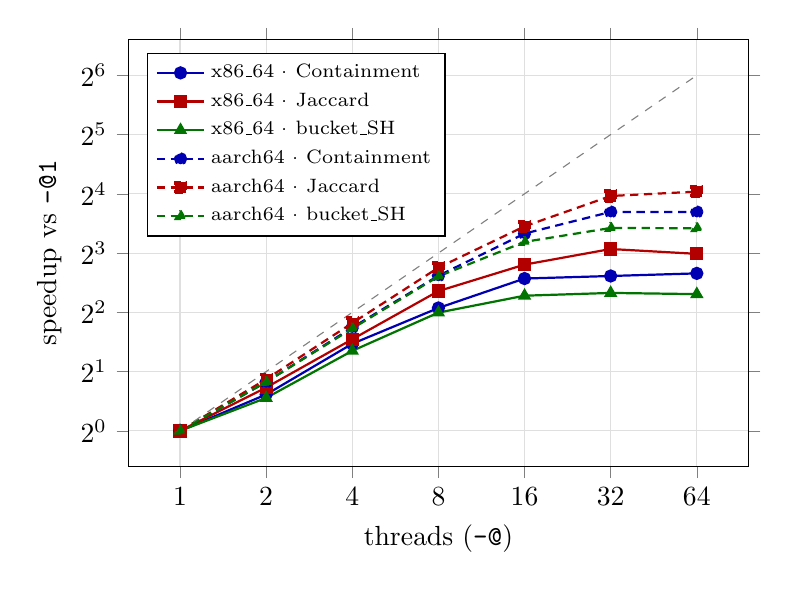
\begin{tikzpicture}
\begin{axis}[
  xlabel={threads (\texttt{-@})},
  ylabel={speedup vs \texttt{-@1}},
  width=0.78\linewidth,
  height=7cm,
  legend pos=north west,
  legend cell align=left,
  legend style={font=\scriptsize},
  grid=major,
  grid style={gray!25},
  tick align=outside,
  xmode=log,
  ymode=log,
  log basis x=2,
  log basis y=2,
  xtick={1,2,4,8,16,32,64},
  xticklabels={1,2,4,8,16,32,64}
]
\addplot[color=blue!70!black,mark=*,solid,thick] coordinates {(1,1.00) (2,1.53) (4,2.77) (8,4.21) (16,5.94) (32,6.12) (64,6.31)};
\addlegendentry{x86\_64 · Containment}
\addplot[color=red!70!black,mark=square*,solid,thick] coordinates {(1,1.00) (2,1.66) (4,2.92) (8,5.13) (16,6.99) (32,8.39) (64,7.93)};
\addlegendentry{x86\_64 · Jaccard}
\addplot[color=green!45!black,mark=triangle*,solid,thick] coordinates {(1,1.00) (2,1.47) (4,2.55) (8,3.99) (16,4.86) (32,5.02) (64,4.95)};
\addlegendentry{x86\_64 · bucket\_SH}
\addplot[color=blue!70!black,mark=*,densely dashed,thick] coordinates {(1,1.00) (2,1.77) (4,3.35) (8,6.14) (16,10.05) (32,12.95) (64,12.95)};
\addlegendentry{aarch64 · Containment}
\addplot[color=red!70!black,mark=square*,densely dashed,thick] coordinates {(1,1.00) (2,1.83) (4,3.53) (8,6.75) (16,10.94) (32,15.60) (64,16.42)};
\addlegendentry{aarch64 · Jaccard}
\addplot[color=green!45!black,mark=triangle*,densely dashed,thick] coordinates {(1,1.00) (2,1.77) (4,3.31) (8,6.09) (16,9.12) (32,10.73) (64,10.70)};
\addlegendentry{aarch64 · bucket\_SH}
\addplot[dashed,gray,forget plot] coordinates {(1,1) (2,2) (4,4) (8,8) (16,16) (32,32) (64,64)};
\end{axis}
\end{tikzpicture}
\caption{Thread scaling on each machine, benchmark B01. Colour is the metric, line style the architecture; the grey diagonal is linear speedup. Each curve is normalised to its own machine's single-threaded time, so the figure compares how well the machines scale, not how fast they are.}
\label{fig:xarch:scaling}
\end{figure}


All measurements are of commit \texttt{\shmCommit}, built with rustc
\shmRustc{} under suite~\shmSuiteVersion, over \shmNumBenchmarks{} benchmarks
$\times$ \shmNumMetrics{} similarity metrics --- \shmNumCells{} cells behind
every range quoted --- at $k=\shmParamK$, $r=\shmParamR$,
$\theta=\shmParamTheta$, $\delta=\shmParamDelta$, $\phi=\shmParamPhi$. The
machines are \texttt{\shmHostX} (\shmArchX, \shmTopologyX, \shmCoresX{}
cores), measured \shmMeasuredX, and \texttt{\shmHostA} (\shmArchA,
\shmTopologyA, \shmCoresA{} cores), measured \shmMeasuredA.

\textbf{Both machines run the same computation.} This is the premise of
everything else, so it is measured rather than assumed. The mapper is
deterministic, so its counters --- reads mapped, confident calls, buckets
seeded, refined and reported --- must be identical on both machines for one
commit. They are, on \shmAgreeCells{} of \shmAgreeTotal{} benchmark--metric
pairs.

\textbf{Speed and memory.} Table~\ref{tab:xarch:speedup} gives the
single-threaded speedup over the C++ on each machine separately; both terms of
each ratio come from the same host, so the host's speed cancels and what
remains is a property of the two programs. It is
\shmSpeedupXMin--\shmSpeedupXMax$\times$ (median \shmSpeedupXMedian$\times$) on
\texttt{\shmHostX} and \shmSpeedupAMin--\shmSpeedupAMax$\times$ (median
\shmSpeedupAMedian$\times$) on \texttt{\shmHostA}. Peak memory is
\shmRssRsMin--\shmRssRsMax~GB against the reference's \shmRssCpp~GB and, unlike
it, is a function of the reads rather than the genome. The reference is built
\texttt{-O3 -march=native -flto}, % lint-ok: upstream build flags, not a measurement
so this is no naive baseline; the advantage widens with input size, and on
inputs small enough to be startup-dominated the C++ still wins. Mapping the
same input takes \shmMapRatioMin--\shmMapRatioMax$\times$ as long on
\texttt{\shmHostA} as on \texttt{\shmHostX}, but the machines differ in far
more than instruction set, so that ratio compares two machines rather than two
architectures.

\textbf{Thread scaling, and where it stops.}
Figure~\ref{fig:xarch:scaling} shows the machines diverging. On the deepest
benchmark (\shmScaleXPeakBench) \texttt{\shmHostX} reaches
\shmScaleXPeak$\times$ at \shmScaleXPeakThreads{} threads then falls back,
while \texttt{\shmHostA} climbs monotonically to \shmScaleAPeak$\times$ at
\shmScaleAPeakThreads{} on \shmScaleAPeakBench. Across the whole matrix the medians are
\shmScaleXKnee$\times$ against \shmScaleAKnee$\times$ at \shmKneeThreads{}
threads, and \shmScaleXCap$\times$ against \shmScaleACap$\times$ at
\shmCapThreads. The gap is not the instruction set: \texttt{\shmHostX} has
\shmTopologyX{} and \texttt{\shmHostA} has \shmTopologyA. The ceiling is
memory-bandwidth contention on the shared index, appearing as soon as a run
spans more than one socket; confining a run to one node with \texttt{numactl}
recovers most of the loss.

\textbf{Accuracy is unchanged, and checked.} On the simulated benchmark, the
only input carrying ground truth, reads land within one read length of their
true position for \shmAccMin--\shmAccMax\% of reads depending on metric, and at
most \shmWrongQMax{} reads under any metric are placed wrongly while reported
as confident --- measured because a regression here must block a merge.

\textbf{Where the time goes.} The costliest stage is \texttt{\shmTopStage}, at
\shmTopStageShare\% of CPU time on average: a pointer-chasing, latency-bound
loop, which is why the profitable changes concerned the shape of the data
rather than the width of the arithmetic. The profile barely moves between
machines --- the largest shift in any stage's share is \shmShiftPP{} percentage
points, in \texttt{\shmShiftStage}, which is input reading.

\section{What did not pay}

Four hypotheses were built or probed at full scale and measured negative; they
are recorded because a negative result nobody writes down gets retried.
Hand-written SIMD sketching loses to the scalar loop, which is load-port bound
at six level-one loads per base, so extra lanes add pressure where there is
none to spare; two-bit packing loses for the same reason from the opposite
direction, removing the wrong two of those loads. Prefetching the pruning
lookups is at best break-even, out-of-order execution already overlapping them.
Per-node index replication --- built five ways, including one bypassing the
allocator for genuinely correct placement --- was slower than doing nothing at
every thread count spanning more than one socket.

\section{Conclusion}

Sketch-based long-read mapping had headroom that was not algorithmic. Sizing
the accumulator by the query instead of the reference, memoising a search that
repeated itself, and decomposing indexing to use the cores a machine has
together give a several-fold improvement in time and close to an order of
magnitude in memory, without changing output by one byte. The remaining ceiling
is the memory system, not the code. Every table, figure and number here is
regenerated from the committed result sets by scripts in the repository, and
continuous integration fails if any drifts from what it reports.

\small
\vspace{0.4em}
\noindent\textbf{Acknowledgements.} \shmContributors{} contributed to this
work as a project member.
\vspace{0.2em}

\begin{thebibliography}{9}
\bibitem{shmap} Ivanov,P. and Medvedev,P. map-shmap: practical long-read mapping with a seed heuristic on sketches. Manuscript in preparation.
\bibitem{mash} Ondov,B.D. \emph{et al.} (2016) Mash: fast genome and metagenome distance estimation using MinHash. \emph{Genome Biol.}, 17, 132.
\bibitem{nthash} Mohamadi,H. \emph{et al.} (2016) ntHash: recursive nucleotide hashing. \emph{Bioinformatics}, 32, 3492--3494.
\end{thebibliography}

\end{document}
